% ============================================================
% Proyecto final — Implementación de alto nivel del Datapath 3
% con unidad de control genérica y motor NEMA 17 en FPGA
%
% Compilar SIEMPRE con:
%   ../../scripts/latexbuild main.tex
% ============================================================
\documentclass[llncs]{llncs}

\usepackage[utf8]{inputenc}
\usepackage[T1]{fontenc}
\usepackage{graphicx}
\usepackage{listings}
\usepackage{hyperref}
\usepackage{xcolor}
\usepackage{booktabs}

\lstdefinestyle{vhdl}{
  language=VHDL,
  basicstyle=\ttfamily\scriptsize,
  keywordstyle=\color{black},
  commentstyle=\color{gray}\itshape,
  stringstyle=\color{black},
  showstringspaces=false,
  breaklines=true,
  frame=single,
  rulecolor=\color{black},
  columns=fullflexible
}
\lstset{style=vhdl}

\begin{document}

\title{Implementación de Alto Nivel del Datapath 3 con Unidad de Control
Genérica y Control de un Motor NEMA 17 en {FPGA}}

\author{Aldo Mauricio Villegas Peralta$^{1}$,%
\and Uriel Lemus Pérez$^{1}$,%
\and Max Ramos Martínez$^{1}$,%
\and Alfredo Ramírez Candia$^{1}$,%
\and Santiago Silverio Flores$^{1}$}

\authorrunning{Villegas Peralta et al.}
\institute{Equipo de Arquitectura de Computadoras,\\
Benemérita Universidad Autónoma de Puebla, Puebla, México\\
\email{\{vp202368617, lp202362797, rm202376182, rc202375947, sf202367190\}@alm.buap.mx}}

\maketitle

\begin{abstract}
Resumen. Se presenta una implementación de nivel RTL del Datapath 3 gobernada
por una unidad de control microprogramada parametrizable: la ROM de
microinstrucciones se pasa como parámetro genérico, de modo que el mismo motor
ejecuta programas distintos sobre hardware distinto. Se validan tres
programas en GHDL: multiplicación \emph{shift--add}, conteo de unos (popcount) y
secuenciación de un motor paso a paso NEMA~17 (Steren MOT-200), con salidas
STEP/DIR por GPIO. Los seis bancos de prueba autochequeados pasan y el
envoltorio de la DE10-Standard se verifica desde sus controles reales.
\end{abstract}

\noindent\textbf{Palabras Clave:} Datapath, Control microprogramado, VHDL,
FPGA, Motor paso a paso.

% ============================================================
\section{Introducción}
\label{sec:intro}

La separación entre camino de datos y unidad de control es uno de los pilares
de la organización de computadoras: el primero ejecuta las microoperaciones y
la segunda determina \emph{qué} microoperación se ejecuta en cada ciclo
~\cite{stallings2016,patterson2017,patterson2021}. En trabajos previos de esta misma unidad se
implementó el Datapath 3 de la asignatura de forma estructural, con una FSM cuyo
programa era una ROM de microinstrucciones escrita explícitamente para cuatro
algoritmos. El proyecto final plantea dar un paso más: mantener ese modelo de
control, pero hacerlo \emph{genérico}, es decir, independiente del algoritmo y
del periférico.

La contribución es doble. Primero, el datapath se describe a nivel de
transferencia de registros (RTL) en una sola arquitectura comportamental, en
lugar de instanciar ocho componentes ~\cite{ashenden2008,brown2009}. Segundo,
la unidad de control recibe la tabla de microcódigo como \texttt{generic}, con
un formato de palabra que incluye campos genéricos admitidos por hardware
ajeno al datapath. Con el mismo VHDL se demuestran tres programas y dos
destinos: el datapath propiamente dicho y un motor NEMA~17 gobernado mediante
un driver externo.

El resto del artículo está organizado así. La Sección~\ref{sec:diseno} describe
la arquitectura, el formato de microinstrucción y las decisiones eléctricas del
motor. La Sección~\ref{sec:propuesta} explica la metodología de verificación y
el mapeo a la placa. La Sección~\ref{sec:simulaciones} muestra las ondas y la
Sección~\ref{sec:resultados} analiza los resultados. Finalmente se presentan
las conclusiones y el apéndice con el código VHDL completo.

% ============================================================
\section{Diseño Teórico}
\label{sec:diseno}

\subsection{Modelo de control microprogramado}

Una unidad de control cableada codifica cada estado en lógica dedicada; una
unidad microprogramada almacena la secuencia de microoperaciones en una memoria
de control y usa un contador de micropaso para recorrerla
~\cite{stallings2016,tanenbaum2013}. Esta última opción fue la adoptada en el
datapath original y es la que se conserva aquí. La diferencia es que la tabla
ya no está escrita dentro de la entidad del control: reside en
\texttt{microcodigo\_pkg.vhd} y se pasa al entity mediante un
\texttt{generic} de tipo arreglo de registros, una construcción admitida por
VHDL-2008 ~\cite{ieee1076-2008,ieee1076-2019,ashenden2008}. En consecuencia, el mismo
\texttt{control\_gen} puede gobernar cualquier máquina que entienda su palabra
de control; basta con proporcionar otra ROM.

La palabra de microinstrucción tiene tres grupos de campos. Los campos de
datapath (\texttt{sel\_sup}, \texttt{wr\_acc}, \texttt{clr\_acc},
\texttt{addr}, \texttt{wr\_rf}, \texttt{op\_alu}, \texttt{sel\_inf},
\texttt{sh}, \texttt{out\_en}) son idénticos a los de la asignatura. Los campos
genéricos (\texttt{g\_dato}, \texttt{g\_wr}, \texttt{g\_en}) transportan un
dato, un estroboscopio de carga y una habilitación de avance hacia el
periférico activo. El tercer grupo controla el flujo: \texttt{salta},
\texttt{salto\_si\_cero}, \texttt{dir}, \texttt{dir\_cero} y \texttt{fin}.
La existencia de dos direcciones de salto (una para salto incondicional y otra
para salto condicional) es una generalización respecto al control original,
que solo tenía una.

El secuenciador es deliberadamente simple: en cada flanco de subida, con
\texttt{enable='1'}, ejecuta la palabra apuntada por \texttt{paso} y calcula el
siguiente valor del contador. Si la palabra tiene \texttt{fin='1'} el
contador se detiene, conservando la última microinstrucción en las salidas; por
eso los bancos de prueba dan un ciclo adicional para que el registro de
destino capture el resultado. Esta forma de describir el control es equivalente
a una FSM de estado = micropaso, pero con el programa como dato
~\cite{wakerly2017,mano2002}.

\subsection{Datapath 3 a nivel RTL}

El módulo \texttt{datapath3\_rtl} mantiene los mismos recursos que el
diagrama de la asignatura: acumulador de 8 bits, banco de 8 registros de 8
bits con un solo puerto de dirección, ALU de ocho operaciones sobre bytes sin
signo (pasar, sumar, restar, incrementar, decrementar, OR, AND y NOT),
multiplexores superior e inferior, desplazador de un bit y detector de cero
~\cite{patterson2014,manokime2000}. Toda la lógica combinacional se calcula en
un bloque y los registros se actualizan en un único proceso síncrono.

El flag \texttt{cero} se toma de la salida del desplazador, es decir, del valor
que se va a escribir en el acumulador. Esto permite que una microinstrucción
calcule un valor y decida el salto en el mismo ciclo, sin etapas de espera.
La ALU no expone acarreo, de modo que los desbordamientos son silenciosos y
modulo 256; los vectores de prueba se eligen dentro de ese rango
~\cite{hennessy2012}.

\subsection{Programa de multiplicación \emph{shift--add}}

El primer programa sustituye la multiplicación por sumas repetidas por el
algoritmo clásico de desplazamiento y adición
~\cite{patterson2017,brown2009}. Se reservan R0 para la constante 1 (necesaria
porque el operando B de la ALU siempre sale del banco de registros), R1 para el
multiplicando $A$, R2 para el multiplicador $B$ y R3 para el producto $P$. En
cada iteración se calcula $B \wedge 1$; si es distinto de cero se acumula
$P \leftarrow P + A$; después se desplaza $A$ a la izquierda y $B$ a la
derecha. Cuando $B$ llega a cero, la última microinstrucción copia $P$ al
acumulador y habilita el buffer de salida.

\subsection{Programa popcount}

El segundo programa cuenta los unos de un byte. Con la misma constante 1 en
R0, repite $c \leftarrow c + (x \wedge 1)$ y $x \leftarrow x \gg 1$ hasta
que $x$ sea cero. Es un ejemplo compacto de cómo los campos genéricos y la ALU
lógica permiten explotar el desplazador, que en los cuatro experimentos
originales solo trabajaba en modo ``pasar'' ~\cite{kleitz2012,pedroni2008}.

\subsection{Motor paso a paso NEMA 17}

El tercer programa no usa el datapath: gobierna el módulo
\texttt{motor\_pasos}. El motor Steren MOT-200 es bipolar de dos fases, con
ángulo de paso de $1.8^\circ$ (200 pasos por vuelta), 3.1~V nominales,
1.7~A por fase y par de retención de 0.59~N\,m
~\cite{steren2026}. El módulo mantiene un contador de pasos cargado desde
\texttt{g\_dato} con \texttt{g\_wr}, avanza una fase con \texttt{g\_en} y
genera el patrón de excitación de dos fases activas
$0011 \rightarrow 0110 \rightarrow 1100 \rightarrow 1001$; el sentido invierte
la secuencia. Un cambio de fase produce un pulso de un ciclo que se conecta a
la entrada STEP del driver.

La FPGA solo suministra señales lógicas de 3.3~V: STEP, DIR, ENABLE (activo a
nivel bajo) y MS1--MS3. La corriente de 1.7~A por bobina la entrega un driver
A4988/DRV8825 con fuente externa y masa común
~\cite{a4988,terasic2018}. Para que las fases sean visibles a simple vista se
usa el módulo \texttt{divisor} de la base común de la placa con un tick de
100~Hz: una vuelta completa tarda aproximadamente dos segundos. El envoltorio
además refleja las fases en LEDR[3:0], de modo que la demostración funciona
también sin conectar el motor.

% ============================================================
\section{Propuesta Experimental}
\label{sec:propuesta}

La validación sigue el flujo del repositorio: los fuentes se analizan con
\texttt{scripts/vhdl-analizar proyecto-final} y cada banco se ejecuta con
\texttt{scripts/vhdl-sim proyecto-final $<$tb$>$}, que produce un VCD en
\texttt{vhdl/proyecto-final/salidas/}. El estándar es VHDL-2008 con
\texttt{--std=08}, y las herramientas son GHDL y GTKWave
~\cite{ghdl-docs,gtkwave-docs}. Los seis bancos usan
\texttt{assert~...~severity~failure} y un \texttt{report~"OK"} final, por lo
que el CI detecta cualquier desviación.

Los bancos cubren cuatro niveles: (i) el secuenciador y sus saltos,
(ii) el datapath RTL con microoperaciones individuales, (iii) cada programa
integrando control y hardware, y (iv) el envoltorio de placa, accionado desde
señales KEY/SW y verificado en los displays y en STEP/DIR. Para simular el
motor en tiempo razonable se incrementa el parámetro \texttt{FREC\_MOTOR\_HZ}
del envoltorio; en la placa se deja en 100~Hz.

La síntesis y la programación se hacen con Quartus Prime Lite por interfaz
gráfica, según la guía del equipo: doble clic en \texttt{top\_placa.qpf},
\texttt{Ctrl+L} y \texttt{Tools $\rightarrow$ Programmer} con el archivo
\texttt{.sof} ~\cite{terasic2018}. Los pines GPIO se asignan según la Tabla
3--11 del manual de la DE10-Standard: GPIO\_0[0] = STEP (PIN\_W15),
GPIO\_0[1] = DIR (PIN\_AK2), GPIO\_0[2] = EN (PIN\_Y16) y GPIO\_0[3--5] =
MS1--MS3.

% ============================================================
\section{Simulaciones de VHDL}
\label{sec:simulaciones}

La Figura~\ref{fig:shift} muestra la ejecución de $4\times3$ en el banco
\texttt{tb\_prog\_shift\_add}. Se observa el recorrido de \texttt{paso} por las
direcciones del programa, los valores sucesivos del acumulador y cómo
\texttt{out\_en} se activa únicamente en la última microinstrucción, cuando
\texttt{dato\_out} entrega el producto $0x0C$.

\begin{figure}[t]
  \centering
  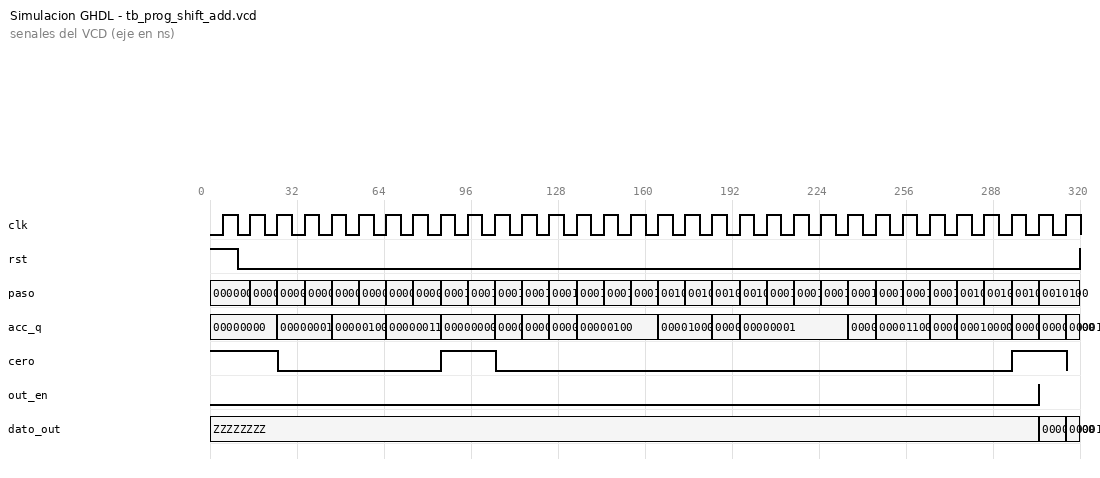
\includegraphics[width=0.95\textwidth]{figuras/shift_add.png}
  \caption{Ondas del programa \emph{shift--add}: $4\times3=12$ (0x0C).}
  \label{fig:shift}
\end{figure}

La Figura~\ref{fig:pop} corresponde a popcount de $0xA5$. Cada iteración
prueba el bit menos significativo con AND, incrementa el contador cuando el bit
está a uno y desplaza el dato a la derecha. El resultado final es 4.

\begin{figure}[t]
  \centering
  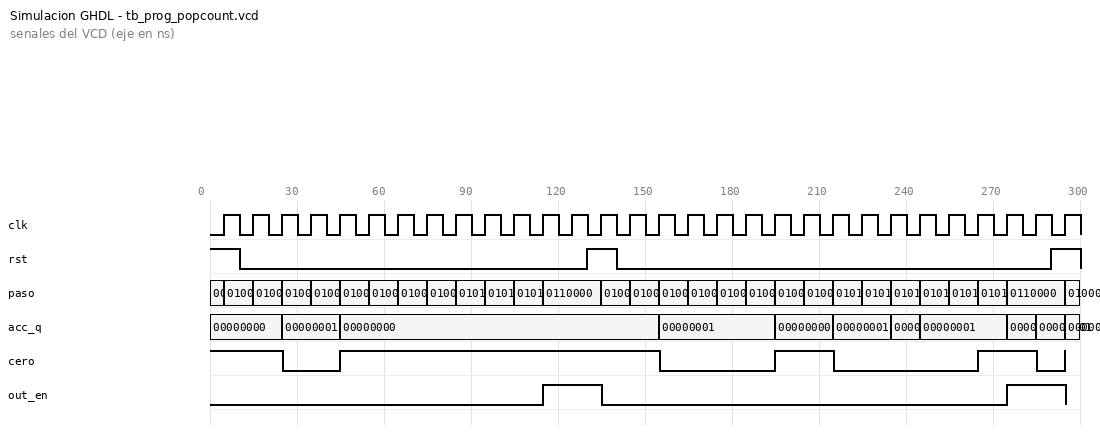
\includegraphics[width=0.95\textwidth]{figuras/popcount.png}
  \caption{Ondas del programa popcount sobre $0xA5$; el conteo termina en 4.}
  \label{fig:pop}
\end{figure}

La Figura~\ref{fig:motor} muestra la secuencia de fases del NEMA 17 y el pulso
STEP asociado a cada cambio. El contador \texttt{pasos\_rest} decrece una vez
por microciclo de avance y el flag \texttt{cero} detiene el programa al
agotarse los pasos.

\begin{figure}[t]
  \centering
  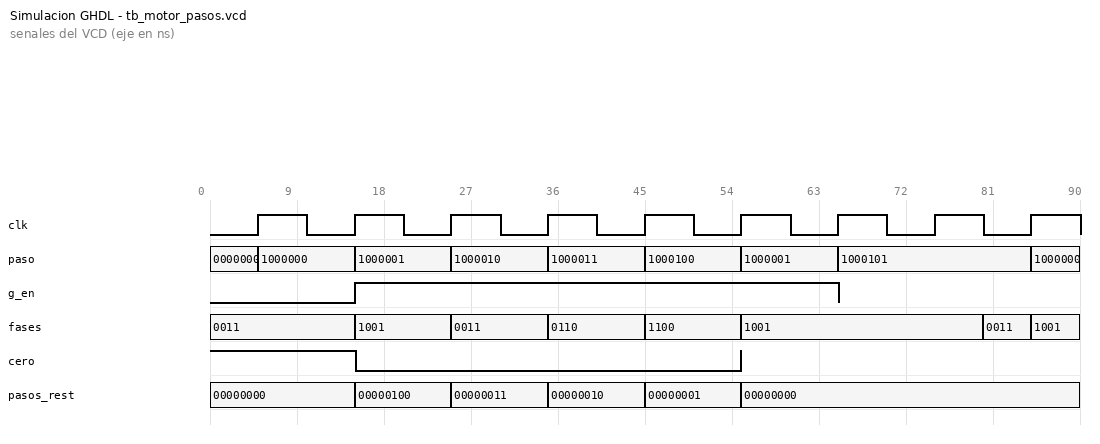
\includegraphics[width=0.95\textwidth]{figuras/motor.png}
  \caption{Secuencia de cuatro fases y pulsos STEP del motor paso a paso.}
  \label{fig:motor}
\end{figure}

La Figura~\ref{fig:top} presenta la simulación del envoltorio completo: la
captura de operandos con KEY0, el paso a estado ocupado y la aparición del
resultado en los displays junto con DIR y STEP.

\begin{figure}[t]
  \centering
  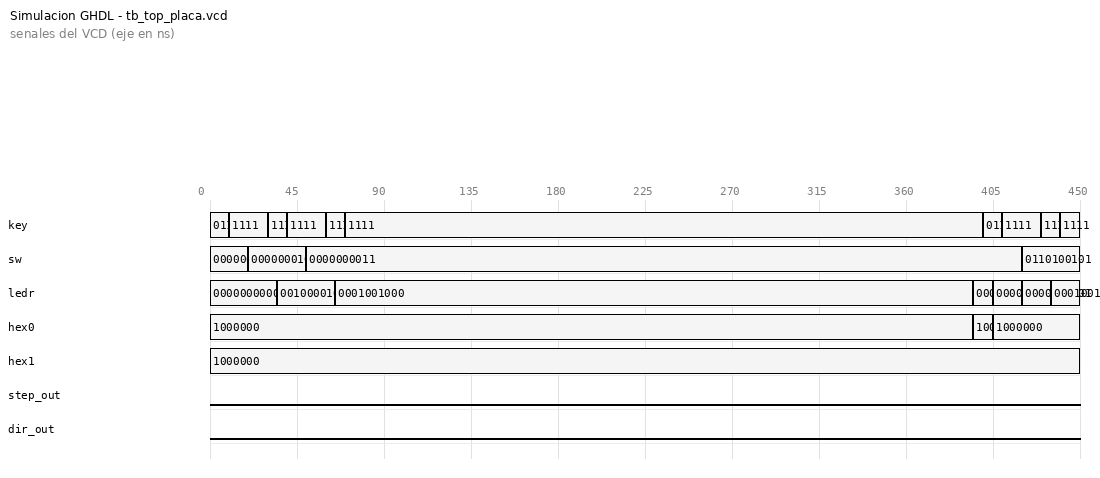
\includegraphics[width=0.95\textwidth]{figuras/top_placa.png}
  \caption{Envoltorio de placa: captura, ejecución y salida de resultados.}
  \label{fig:top}
\end{figure}

% ============================================================
\section{Resultados}
\label{sec:resultados}

\subsection{Verificación funcional}

Los seis bancos de prueba terminan correctamente. El banco del secuenciador
comprueba las tres secuencias de \texttt{paso}, incluidos los saltos
condicionales, y verifica que \texttt{enable='0'} congela el contador. El banco
del datapath valida carga, escritura y lectura del banco, las ocho operaciones
de la ALU, los cuatro códigos del desplazador, el flag de cero y el buffer en
alta impedancia. Los bancos de aplicación comprueban los resultados y los
tiempos de ejecución.

\begin{table}[t]
\centering
\caption{Resultados del programa \emph{shift--add}.}
\label{tab:shift}
\begin{tabular}{@{}llr@{}}
\toprule
Entrada & Resultado & Microciclos \\
\midrule
$4\times3$ & 12 & 30 \\
$5\times5$ & 25 & 38 \\
$15\times15$ & 225 & 52 \\
$0\times7$ & 0 & 41 \\
$1\times255$ & 255 & 96 \\
\bottomrule
\end{tabular}
\end{table}

La Tabla~\ref{tab:shift} resume los cinco vectores de multiplicación. El número
de microciclos crece con el número de bits uno del multiplicador, porque cada
bit a uno añade una adición; el caso $1\times255$ es el más largo con 96
microciclos. La Tabla~\ref{tab:pop} recoge los seis vectores de popcount; de
nuevo, el tiempo depende del número de unos y del número de desplazamientos
necesarios hasta agotar el byte.

\begin{table}[t]
\centering
\caption{Resultados del programa popcount.}
\label{tab:pop}
\begin{tabular}{@{}llr@{}}
\toprule
Entrada & Unos & Microciclos \\
\midrule
0x00 & 0 & 11 \\
0x01 & 1 & 14 \\
0x80 & 1 & 49 \\
0xA5 & 4 & 58 \\
0xF0 & 4 & 58 \\
0xFF & 8 & 70 \\
\bottomrule
\end{tabular}
\end{table}

\subsection{Motor NEMA 17}

El banco \texttt{tb\_motor\_pasos} verifica la secuencia de fases en ambos
sentidos, con 1, 4 y 8 pasos y con cero pasos. En todos los casos el contador
termina en cero y el número de transiciones de fase coincide con el de pasos
solicitados. El envoltorio genera exactamente cuatro pulsos STEP para una
petición de cuatro pasos, con DIR igual al sentido elegido y ENABLE a nivel
bajo. La Tabla~\ref{tab:motor} recoge la secuencia de excitación.

\begin{table}[t]
\centering
\caption{Secuencia de fases de dos bobinas activas.}
\label{tab:motor}
\begin{tabular}{@{}ccccc@{}}
\toprule
Fase & Adelante & Atrás & Patrón & Ángulo \\
\midrule
0 & 0 & 3 & 0011 & $0^\circ$ \\
1 & 1 & 2 & 0110 & $1.8^\circ$ \\
2 & 2 & 1 & 1100 & $3.6^\circ$ \\
3 & 3 & 0 & 1001 & $5.4^\circ$ \\
\bottomrule
\end{tabular}
\end{table}

\subsection{Discusión}

Los resultados confirman que la generidad del control no cuesta funcionalidad:
un mismo \texttt{control\_gen} ejecuta dos programas sobre el datapath y uno
sobre un periférico distinto. El coste es una palabra de control más ancha y una
ROM con campos que cada hardware interpreta de forma distinta. La decisión de
usar \texttt{enable} como tick compartido evita que el motor avance en cada
ciclo de 50~MHz, un error que se detectó y corrigió durante la verificación
del envoltorio.

Las limitaciones son las heredadas del diseño original: aritmética módulo 256
sin acarreo, un solo puerto en el banco de registros y ausencia de realimentación
mecánica en el motor (control en lazo abierto). Como trabajo futuro se plantea
añadir micropaso con los pines MS y un sensor de posición para cerrar el lazo.

% ============================================================
\section{Conclusiones}
\label{sec:conclusiones}

Se cumplió el objetivo: existe una descripción RTL del Datapath 3 y una unidad
de control microprogramada parametrizable que gobierna tres programas y dos
hardware distintos, validada con seis bancos autochequeados y llevada a la
DE10-Standard con salidas STEP/DIR para un NEMA~17. El uso de una ROM pasada
como \texttt{generic} hace explícita la diferencia entre control cableado y
control microprogramado: el algoritmo es datos, no lógica. La verificación a
nivel de envoltorio demostró además detalles que la simulación aislada no
revela, como la necesidad de sincronizar el avance del motor con el tick de
habilitación. El siguiente paso natural es ampliar la familia de
microprogramas y explorar el micropaso para mejorar la resolución angular.

% ============================================================
\bibliographystyle{splncs04}
\bibliography{referencias}

% ============================================================
\appendix
\section{Código VHDL}
\label{app:codigo}

\lstinputlisting[caption={microcodigo\_pkg.vhd --- formato de la
microinstrucción y programas}, label=lst:microcodigo]
{../../vhdl/proyecto-final/src/microcodigo_pkg.vhd}

\lstinputlisting[caption={control\_gen.vhd --- secuenciador microprogramado
genérico}, label=lst:control]
{../../vhdl/proyecto-final/src/control_gen.vhd}

\lstinputlisting[caption={datapath3\_rtl.vhd --- camino de datos a nivel RTL},
label=lst:datapath]
{../../vhdl/proyecto-final/src/datapath3_rtl.vhd}

\lstinputlisting[caption={motor\_pasos.vhd --- controlador del NEMA 17},
label=lst:motor]
{../../vhdl/proyecto-final/src/motor_pasos.vhd}

\lstinputlisting[caption={top\_placa.vhd --- envoltorio de la DE10-Standard},
label=lst:top]
{../../vhdl/proyecto-final/fpga/top_placa.vhd}

\end{document}
